\begin{figure}[h]
\centering
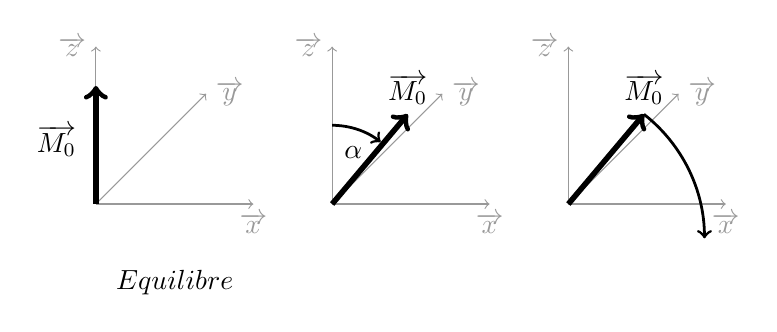
\begin{tikzpicture}

%% Partie 1
   \path [->,color = gray!80] (0,0) edge (0,2);
   \path [->,color = gray!80] (0,0) edge (2,0);
   \path [->,color = gray!80] (0,0) edge (1.4,1.4);
   
   \draw [color = gray!80] (0,2) node[left] {$\overrightarrow{z}$};
   \draw [color = gray!80] (2,0) node[below] {$\overrightarrow{x}$};
   \draw [color = gray!80] (1.4,1.4) node[right] {$\overrightarrow{y}$};
   
   %dessin M0
   \path [->,line width=2pt] (0,0) edge (0,1.5);
   \draw (-0.5,0.8) node {$\overrightarrow{M_0}$};
      \draw (1,-1) node {$Equilibre$};
   
%% partie 2
\def\PositionB{3}
   \path [->,color = gray!80] (0+\PositionB,0) edge (0+\PositionB,2);
   \path [->,color = gray!80] (0+\PositionB,0) edge (2+\PositionB,0);
   \path [->,color = gray!80] (0+\PositionB,0) edge (1.4+\PositionB,1.4);
   
   \draw [color = gray!80] (0+\PositionB,2) node[left] {$\overrightarrow{z}$};
   \draw [color = gray!80] (2+\PositionB,0) node[below] {$\overrightarrow{x}$};
   \draw [color = gray!80] (1.4+\PositionB,1.4) node[right] {$\overrightarrow{y}$};
   
   %Dessin M0
   \draw [->,line width=1pt] (0+\PositionB,1) arc (90:52:1);
   
   \draw (1.5*0.18+\PositionB,1.5*0.30) node [above] {$\alpha$};

   \path [->,line width=2pt] (0+\PositionB,0) edge (\PositionB+1.5*0.64,1.5*0.76);
   \draw (1.5*0.64+\PositionB,1.5*0.76) node [above] {$\overrightarrow{M_0}$};

%% partie 3
\def\PositionB{6}
   \path [->,color = gray!80] (0+\PositionB,0) edge (0+\PositionB,2);
   \path [->,color = gray!80] (0+\PositionB,0) edge (2+\PositionB,0);
   \path [->,color = gray!80] (0+\PositionB,0) edge (1.4+\PositionB,1.4);
   
   \draw [color = gray!80] (0+\PositionB,2) node[left] {$\overrightarrow{z}$};
   \draw [color = gray!80] (2+\PositionB,0) node[below] {$\overrightarrow{x}$};
   \draw [color = gray!80] (1.4+\PositionB,1.4) node[right] {$\overrightarrow{y}$};
	
	\path [->,line width=2pt] (0+\PositionB,0) edge (\PositionB+1.5*0.64,1.5*0.76);
   \draw (1.5*0.64+\PositionB,1.5*0.76) node [above] {$\overrightarrow{M_0}$};

	%dessiner ellipse
	\draw [->,line width=1pt] (1.5*0.64+\PositionB,1.5*0.76) arc (52:0:2);
   
\end{tikzpicture}

\caption[Angle de bascule]{Représentation de l'effet d'une impulsion RF sur une aimantation induite par un champ aligné selon $\overrightarrow{z}$, à l'équilibre, après excitation et durant l'état de précession.}
\end{figure}
